% vim:ft=tex

\section{Evaluation of Hadoop Distributions}

This chapter shows a general conducted comparison of Hadoop distributions which are dominating the big
data market. Since it is necessary for our data science project to compute in a parallel and efficient fashion, such a comparison helps us to identify the right distribution. Firstly, an overview of the identified distributions with its features and pricing tiers will be showed. Afterwards we will declare some important criteria for our project based on an extensive research of internet blogs and manufacturer websites. Then a weighting of these criteria will be done. These criteria will be used to evaluate the different Hadoop distributions. The resulting evaluation matrix shows that Hortonworks might be the best distribution for our data science problem. However, a detailed look at the performance criterion shows us that MapR is the most most powerful in five5 out of six cases. For this performance comparison, evaluation results of various MapReduce jobs found on the Internet are used. Hence, in a pure performance comparison MapR would win over Hortonworks, but in an overall comparison Hortonworks convinces more. To round off the
evaluation, a test implementation of Hortonworks was carried out on the four virtual machines procured for
this purpose where some simple MapReduce jobs are carried out.
\subsection{Hadoop Distributions Overview}\label{hd}
For the first part of the evaluation, a search for widespread Hadoop distributions was conducted \citep{hadoopvendors,forrester,comparison2014,Cloudera,M.Heo2015}.
As the table~\ref{tab:distributions} below shows, seven noteworthy distributions were found.
%\hspace{-2.5cm}
\begin{table}[H]
%\centering
\hspace{-3.3cm}
\begin{tabular}{|p{4.4cm}|p{6.2cm}|p{4cm}|p{4cm}|}
	\hline
	\textbf{Hadoop \newline Distribution} & \textbf{Features} & \textbf{ Pricing Gear}  & \textbf{ Hadoop \newline Ecosystem}\\ \hline
	Apache Hadoop 3.1.1
\href{http://hadoop.apache.org/}{hadoop.apache.org} & 
\begin{itemize}[noitemsep,leftmargin=*]
   \item No extra tools
   \item Blank installation of Apache Hadoop (HDFS, YARN and Hadoop Web UI)
\end{itemize}
& Open Source 100\% & Has to be
installed
manually \citep{apachehadoop}\\ \hline
Cloudera CDH (v5.15.0)
\href{https://www.cloudera.com/}{www.cloudera.com} & \begin{itemize}[noitemsep,leftmargin=*]
   \item Oldest distribution
   \item Very polished
   \item Comes with good (and proprietary)
tools to install and manage a Hadoop
cluster: \begin{itemize}
\item Cloudera Manager for managing
and monitoring clusters \citep{Cloudera2018a}.
\item Cloudera Search (Free-Text) on
Hadoop \citep{Cloudera2018}.
\item Apache Crunch framework for
MapReduce Pipelines \citep{Cloudera2018}.
\end{itemize}
\end{itemize} &Freemium (Cloudera Manager require license). Also source code is not fully available and enterprise edition has 60 trial-day \citep{D.Kumar2016}. Final costs may depend on cluster size \citep{Cloudera}.  &Accumulo,Flume, HBase, HCatalog, Hive, HttpFS, HUE, Impala, Kafka, KMS, Mahout, Oozie, Pig, Sentry, Snappy, Spark, Sqoop, Parquet, Whirr, ZooKeeper \citep{Cloudera2018a,Cloudera2018}\\ \hline
\end{tabular}
%\caption{Vergleich ausgewählter Column Family Datenbanken (eigene Darstellung)}
\label{tab:distributions}
\end{table}
%end first table!
\vspace{-2.5cm}
\begin{table}[H]
%\centering
\hspace{-3.3cm}
\begin{tabular}{|p{4.4cm}|p{6.2cm}|p{4cm}|p{4cm}|}
	\hline
	\textbf{Hadoop \newline Distribution} & \textbf{Features} & \textbf{ Pricing Gear}  & \textbf{ Hadoop \newline Ecosystem}\\ \hline
Hortonworks Data
Platform (HDP3.0.1)
\href{https://hortonworks.com/}{www.hortonworks.com} &\begin{itemize}[noitemsep,leftmargin=*] \item Newer distributions
\item Tracks Apache Hadoop closely
\item Comes with standard and open source
tools for managing clusters:
\begin{itemize}
\item Improved HDFS in HDP 2.0:
automated fail over with a hot
standby and full stack resiliency
\citep{Hortonworks2018c}.
\item Ambari for managing and monitoring clusters. \item Includes almost all Hadoop
extensions from the Apache
foundation \citep{Hortonworks2018c}.
\end{itemize}
\end{itemize} & Open Source, optional enterprise paid support \citep{D.Kumar2016} &Atlas, HBase, HDFS, Hive Metastore, HiveServer2, Hue, Spark, Kafka, Knox, Oozie, Ranger, Storm, WebHCat, YARN, SmartSense, ZooKeeper \citep{Hortonworks2018b} \\ \hline
MapR 6.1 \href{https://mapr.com/} {www.mapr.com} &\begin{itemize}[noitemsep,leftmargin=*] 
\item Uses own HDFS (MapR-FS)
\item Integrates own database systems (MapR-DB seven times faster than HBase)
\item Mostly used for big big data projects
\item Free from Single Point of Failures
\item Offers Mirroring and Snapshotting
\item Might be the fastest Hadoop distribution 
\item MapR supports backward compatibility across multiple version of projects
\item Supports a global event replication for streaming at IoT scale (MapR-ES)
\end{itemize}& Freemium \citep{MapR2018b}:Community Edition contains no high availability, no disaster recovery and no global replication for streaming data.& AsyncHBase, Cascading, Drill, Flume, HBase Client and MapR Database, Binary Tables, Spark, HCatalog, Hive, HttpFS, Hue, Impala MapR Event Store For Apache Kafka Clients and Tools, Myriad, OpenStack, Manila, Oozie, Pig, Sentry, Spark, Sqoop, MapR Object Store with S3- Compatible API\citep{MapR2018a}\\ \hline
\end{tabular}
\label{tab:distributions}
\end{table}
%end second table!
\begin{table}[H]
\hspace{-3.3cm}
\begin{tabular}{|p{4.4cm}|p{6.2cm}|p{4cm}|p{4cm}|}
	\hline
	\textbf{Hadoop \newline Distribution} & \textbf{Features} & \textbf{ Pricing Gear}  & \textbf{ Hadoop \newline Ecosystem}\\ \hline
Intel
\href{https://http://hadoop.intel.com/}{www.hadoop.intel.com}
&\begin{itemize}[noitemsep,leftmargin=*] 
\item Partnered with Cloudera \citep{MervAdrian2017}
\item Encryption support
\item Hardware acceleration added to layers of stack to boost performance
\item Admin tools to deploy and manage Hadoop
\end{itemize}&
Premium (90 days trial) & Offers same
services as
Cloudera. \\ \hline
Pivotal HD
 \href{https://gopivotal.com//} {www.gopivotal.com} &\begin{itemize}[noitemsep,leftmargin=*] 
\item Partnered with Hortonworks \citep{MervAdrian2017}
\item Fast SQL on Hadoop
\item Proprietary Software \citep{Pivotal2018}:
\begin{itemize}
\item Pivotal DataLoader
\item USS (external file system)
\item Spring Data
\item Pivotal ADS-HAWQ (parallel SQL query engine)
\end{itemize}
\end{itemize}& Premium &Offers same services as Hortonworks.\\ \hline
IBM Open Platform
\href{https://www.ibm.com/de-de/?ar=1}{www.ibm.com}&\begin{itemize}[noitemsep,leftmargin=*] 
\item Partnered with Hortonworks \citep{MervAdrian2017}
\item Proprietary tools:
\begin{itemize}
\item IBM Big SQL allows concurrent process of Hive, HBase and Spark and other sources using a single database connection \citep{MervAdrian2017}.
\item IBM BigInsights v4.2 provides Text-Analytics module \citep{I.K.Center2018}.
\end{itemize}
\item Highly compatible to other IB products.
\end{itemize}
&Free for non-commercial purposes, optional enterprise paid support \citep{IBMAnalytics2018}
& Offers same services as Hortonworks.\\ \hline
\end{tabular}
\caption{Overview of Hadoop distributions}
\label{tab:distributions}
\end{table}
\noindent It is worth to mention that each Hadoop distribution in table \ref{tab:distributions} comes up with a minimum of services from the Apache foundation: \ac{yarn}, \ac{hdfs}, Hive, Pig, HBase, Kafka, Storm, Mahout, HCatalog... But they may use a proprietary implementation of them e.g. MapR uses own HDFS instead of Apache HDFS implementation. It is also worth to note that a few cloud providers are offering Hadoop cluster services over their platforms. For instance, Microsoft Azure provides with HDInsight a full manageable Hadoop respectively Spark Cluster \citep{Microsoft2018}. The user could profit from fast provisioning and also from less costs since no on-prem hardware cluster infrastructure is required. Therefore, Hadoop (or better Spark) by Cloud Computing is also a noteworthy option for our data science project in the future, although it may be over sized at the moment. It is worth to mention that each Hadoop distribution in table \ref{tab:distributions} comes up with a minimum of services from the Apache foundation: YARN, HDFS, Hive, Pig, HBase, Kafka, Storm, Mahout, HCatalog etc. But they may use
a proprietary implementation of them e.g. MapR uses own HDFS instead of Apache HDFS implementation. 
It is also worth to note that a few cloud providers are offering Hadoop cluster services over their platforms. 
For instance, Microsoft Azure provides with HDInsight a full manageable Hadoop respectively Spark Cluster
\citep{Microsoft2018}. The user could profit from fast provisioning and also from less costs since no on-prem hardware
cluster infrastructure is required. Therefore, Hadoop (or better Spark) by Cloud Computing is also a
noteworthy option for our data science project in the future, although it may be over sized at the moment.\\\\
Nevertheless, Intel, ERM/Pivotal and IBM partnered with Hortonworks or Cloudera \ref{tab:distributions}. These vendors therefore have the same extensions as their partners offer, but also can provide exclusive tools for users (e.g. IBM Big SQL \citep{MervAdrian2017}). If we take this into account, we find that there are mainly 3 different Hadoop distributions: Cloudera with CDH, Hortonworks with its \ac{hdp} and MapR with its own HDFS. In addition to the distributions shown in \ref{tab:distributions}, there are many other Hadoop distributions such as Altiscale from SAP or Elastic MapReduce from Amazon. Both run only in a cloud environment. The Forrester Wave shows also the three global players Cloudera, Hortonworks and MapR (see \ref{pic:forrester}). Since cloud solutions do not play a role for this use case, Microsoft, Google or Amazon will not be considered.
\begin{center}
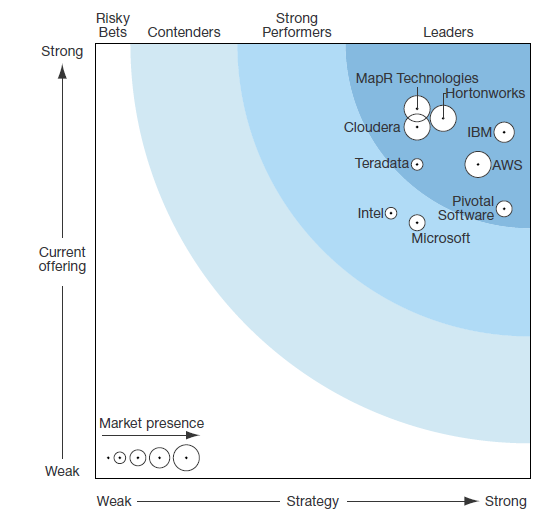
\includegraphics[width=0.8\textwidth]{img/figure1}
\captionof{figure}{Forrester Wave of Hadoop Distributions \citep{forrester}}\label{pic:forrester}
\end{center}
As we can see from 
\ref{pic:forrester} 
the three mentioned Hadoop distributions are building a cluster and Cloudera
even overlaps with MapR slightly. That means, they are providing similar products and enjoy a similar
market position. From the Forrester Wave (\ref{pic:forrester}) we can derive that MapR seems to have the best offering. However, since we want to use one of them for our analytics project we have to dig a step deeper and make a decision based on well-defined criteria.
\subsection{Definition of criteria}
Hadoop distributions are rated using selected criteria, with scores ranging from 1 (very poor) to 5 (very
good). Based on the research carried out, the following 20 clear criteria can be determined:
\begin{table}[H]
\hspace{-1.6cm}
\begin{tabular}{|l|l|}
\hline
\textbf{Criterion}             & \textbf{Description}                                                                                                                                                     \\ \hline
Batch Processing               & \begin{tabular}[c]{@{}l@{}}Batch process jobs can run without any end-user\\ interaction or can be scheduled to start up on their own\\ as resources permit\end{tabular} \\ \hline
Cloud Support                  & Cloud compatibility of Hadoop distributions                                                                                                                              \\ \hline
Cluster Scalability            & \begin{tabular}[c]{@{}l@{}}Creating new clusters ad-hoc and set up cluster size\\ (e.g. 4,8 or 12 nodes)\end{tabular}                                                    \\ \hline
Data querying possibilities    & \begin{tabular}[c]{@{}l@{}}Ways to query Hadoop with SQL (e.g. Hive, Stinger,\\ Spark SQL,...)\end{tabular}                                                              \\ \hline
Database Support               & \begin{tabular}[c]{@{}l@{}}Additional databases in Hadoop (e.g. PostgreSQL,\\ MongoDB, HBase, Impala etc.)\end{tabular}                                                    \\ \hline
Disaster-Discovery             & \begin{tabular}[c]{@{}l@{}}There is a fallback option available in case of\\ unexpected Hadoop errors\end{tabular}                                                       \\ \hline
Ease of Use                    & The complexity of the usage of the Hadoop distribution                                                                                                                   \\ \hline
High-Availability               & \begin{tabular}[c]{@{}l@{}}Self-healing across multiple services or single failure\\ recovery (i.e. fail-over clusters)\end{tabular}                                     \\ \hline
Install complexity             & \begin{tabular}[c]{@{}l@{}}Is there a simple installation routine or does it require\\ lot of manual configuration (e.g. Multi node Cluster...)?\end{tabular}             \\ \hline
Licensing and Pricing          & Cost model of Hadoop distributions                                                                                                                                       \\ \hline
ML support                     & \begin{tabular}[c]{@{}l@{}}Providing interface for enlarged machine learning tasks\\ (e.g. Spark MLlib...)\end{tabular}                                                  \\ \hline
Operating System Support       & Guaranteed and certified OS compatibility                                                                                                                                \\ \hline
Performance                    & \begin{tabular}[c]{@{}l@{}}Cluster performance in case of parallelized MapReduce\\ Jobs\end{tabular}                                                                     \\ \hline
Programming Language Support   & \begin{tabular}[c]{@{}l@{}}Support of data science programming languages\\ (Python and R)\end{tabular}                                                                   \\ \hline
Streaming Analytics            & \begin{tabular}[c]{@{}l@{}}Vendor offering real-time analytics capabilities (e.g. IoT\\ platform hub..)\end{tabular}                                                     \\ \hline
Support of secondary services  & Services on top of Hadoop (e.g. Zookeeper, Spark...)                                                                                                                     \\ \hline
Third party module integration & Usage of additional components from other vendors                                                                                                                        \\ \hline
User Support/Community         & How fast is the response in the community?                                                                                                                               \\ \hline
Expertise                      & Experience with Hadoop (life time of company, ...)                                                                                                                       \\ \hline
\end{tabular}
\caption{Definition of criteria}
\label{tab:criteria}
\end{table}
\noindent The weight scale ranges from 1 (trivial) to 4 (very important), with the focus on our Santander Bicycle project. This means that cloud support, for example, is a crucial criterion in many use cases, but has only little importance for our project which leads to a trivial weight. A percentage weighting is not applied because 20 criteria would result in a fine-granular distribution (which is not good to read at all). Therefore, absolute values are used for the comparison \ref{pic:matrix} in the next section.
\subsection{Weighted evaluation matrix}\label{weight}
As already mentioned in Section \ref{hd}, the three major Hadoop distributions are: Cloudera CDH 5.15.0,
Hortonworks HDP 3.0.1 and MapR 6.1.0. With regard to the defined comparison criteria, a weighted
decision matrix can be mapped. At the same time, this matrix represents the starting point for the decision of a Hadoop distribution. It cannot be denied that a certain degree of subjectivity is included in the evaluation (table \ref{tab:criteria}). In addition, only free editions are compared. For example, if a feature only exists in the premium version, this feature will be rated one (worst) since we don’t want to spend money.
\begin{center}
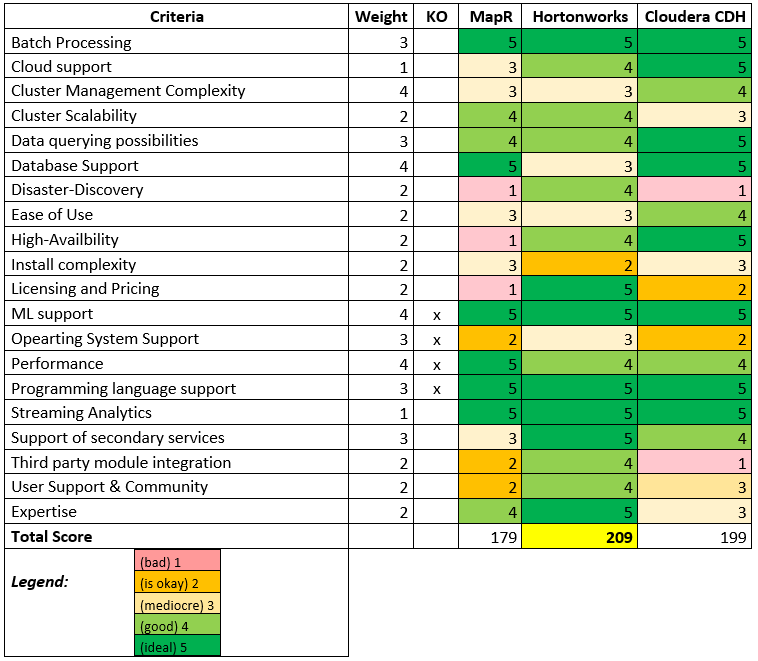
\includegraphics[width=1.0\textwidth]{img/matrix}
\captionof{figure}{Weighted Comparison Table of Hadoop Distributions}\label{pic:matrix}
\end{center}
The comparison in figure \ref{pic:matrix} clearly shows that there are almost no significant differences between the selected distributions. Although there are a few deviations such as disaster-discovery or pricing model, the overall distribution of points is relatively the same. From the comparison matrix it can be deduced that Hortonworks HDP achieves the highest score and is probably the best option for our project at the moment. It is possible that after the first test phase (see chapter \ref{intallhadoop}), it turns out that the distribution is not convenient after all which may require to update the evaluation matrix. Therefore figure \ref{pic:matrix} can be considered as a continuous iterative updateable weighted comparison matrix that will likely be updated on further sprints. Another representation of the evaluated Hadoop distributions, a spider chart may be appropriate as it makes it easier to read and to identify outliers or similarities even quicker as with a raw table.
\begin{center}
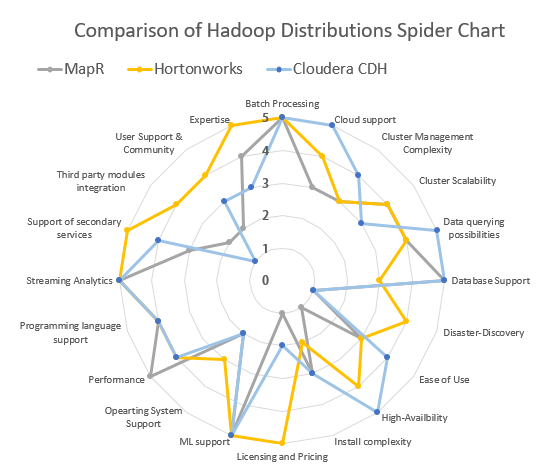
\includegraphics[width=1.0\textwidth]{img/spider}
\captionof{figure}{Spider Chart of compared Hadoop Distributions}\label{pic:spider}
\end{center}
The KO-criteria from figure \ref{pic:matrix} are all satisfied by the selected Hadoop vendors. One criterion that stands out is the license model, which was rated with 1 point for MapR and 2 points for Cloudera. This is due to the fact that the price models of both vendors are not transparent. So Cloudera offers a free community edition but to use the Cloudera Manager (the real strength of Cloudera) you have to pay again. Only Hortonworks offers a complete Open Source package with except the Hortonworks business support is fee required. However, Hortonworks has a very active community as well. MapR comes off worst with the criterion “Support of secondary services”, because there is no Spark and
HBase support in the "Converged Community Edition" \citep{MapR2018b}, but both are important Hadoop components for our project. So if we wanted to use MapR, we would have to use the paid version. There are also some other differences in figure \ref{pic:spider} such as Disaster-Recovery which is only on Hortonworks’s HDP completely free. An interesting aspect of the comparison is the performance criterion where MapR has the most points. Since this criterion is a KO-criterion that means it is a very important component for our project, it makes sense to examine the performance comparison between the distributions in a more detailed fashion.
\subsection{Performance Comparison with micro benchmarks}
For a performance comparison it is good to know how fast they compute when running in a
concurrent mode. For this task MapReduce Jobs like WordCount or \ac{dfsio} Read/Write might be helpful. Following figures are extracted from a sophisticated evaluation work by Altoros \citep{altoros}.
\begin{center}
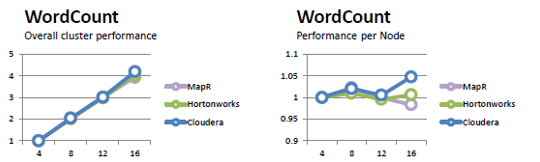
\includegraphics[width=1.0\textwidth]{img/bench1}
\vspace{0.1cm}
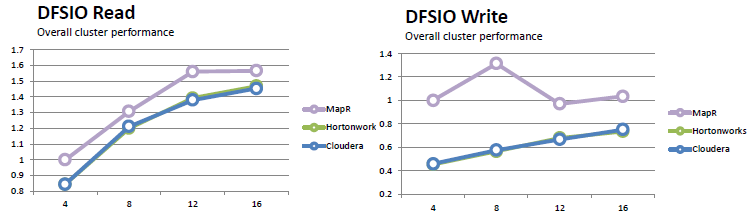
\includegraphics[width=1.0\textwidth]{img/bench2}
\captionof{figure}{Micro benchmarks on DFSIO / WordCount MapReduce Jobs}\label{pic:benchmarks}
\end{center}
For the performance comparison of figure \ref{pic:benchmarks} Hadoop cluster each one with 16 nodes have been established in order to measure computation time. An interesting point is that all three Hadoop distributions almost achieve the same overall speed on the famous WordCount MapReduce job. But if we look at the performance per node then there is a small difference between them. This could be due to a certain error rate in the execution of the job. If the same test were repeated, the results would be negligibly different. The DFSIORead/Write (figure \ref{pic:benchmarks}) job shows MapR is definitely faster than Hortonworks and Cloudera. The reason for
this might be the fact that MapR uses its own HDFS which is according to the vendor seven times faster
than the original one from Apache. This is the reason why it gets five points in the evaluation matrix (see table \ref{tab:criteria}) whereas other ones only reach four points. Hortonworks and Cloudera seems to have the same performance on the DFSIO job because both using Apache HDFS.\\In overall, Hortonworks HDP wins the competition for the moment, because they have the longest experience and are completely compatible with secondary services. Based on the evaluation matrix from chapter \ref{weight} and the performance measurements, it can be deduced that MapR is the most powerful Hadoop distribution on the market today, but when considering the other criteria, Hortonwork's Hadoop is simply more convincing. Especially the complete Open Source guarantee at Hortonworks is a decisive criterion for the choice of this distribution.\\Beside from the comparison, we would generally recommend to use rather Spark than Hadoop since Spark is around 100 times faster due to in-memory processing. Also Spark provides the most important libraries (ML, Streaming, etc) for data science and works well on top of Hadoop (thanks YARN). It can even be installed in a standalone manner, even though it doesn’t benefit from distributive multi mode computing.
\subsection{Installation of sample Hadoop Distribution}\label{intallhadoop}
Hortonworks offers a configurator on their website that can be used to check products, operating systems,
databases, browsers, JDKs and supported processors. It is noticeable that Ubuntu is only supported up to
16.04 LTS. However, our VMs are already v.18.4 LTS. This means Hortonworks does not official support
our installed OS \citep{Hortonworks2018a}. Also Cloudera CDH 5.15 \citep{Cloudera2018b} and the newest MapR 6.1 distribution \cite{MapR2018} only support Ubuntu 16.04 LTS (Xenial). Anyway, it is still a worth a try to set up \acs{hdp} Cluster on our virtual machines since the vendors are not explicitly warning Ubuntu 18.04 is not supported. So it may work. For the installation of HDP 3.0.1 the Ambari Wizard \citep{Hortonworks2018} will be used.\\First of all, we have to configure the \textbf{etc/hosts} since every node in the cluster must be able to communicate with each other. The hosts file should look like this:
\begin{figure}[H]
\hspace{-1.3cm}
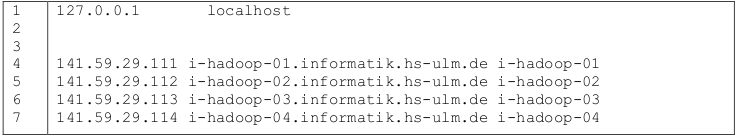
\includegraphics[width=1.2\textwidth]{img/etchost}
\captionof{figure}{etc/hosts configuration file}\label{pic:etchost}
\end{figure}
\noindent After that step, it is necessary to add public key authentication with SSH. The master node (\textbf{i-hadoop-01}) should login to its worker nodes without using a password. We can achieve this goal by generating a private / public key pair and distribute the public key to the 3 worker nodes by using \textbf{ssh-copy-id} command. Also for using Ambari the Hadoop user need sudo execution without password. Adding an additional line to \textbf{visudo} configuration file should solve that issue. At next, all nodes need to have Java installed. Since Ubuntu 18.04 doesn’t come up with a default Java JDK
we install Oracle JDK 1.8 manually on each node. After that it is time to download the Ambari repository
file to a directory on our Hadoop master host. The Ambari v. 2.7.1.0 is used for installation. With the command \textbf{apt-get install ambari server} the server will be installed on i-hadoop-01. Afterwards, we can start the server. Now we can go to the Ambari surface via following link: \href{http://i-hadoop-01.informatik.hs-ulm.de:8080}{http://i-hadoop-01.informatik.hs-ulm.de:8080}. The default login credentials are \textbf{admin admin}. After successful login, the real installation process begins.
\begin{figure}[H]
\hspace{-2.3cm}
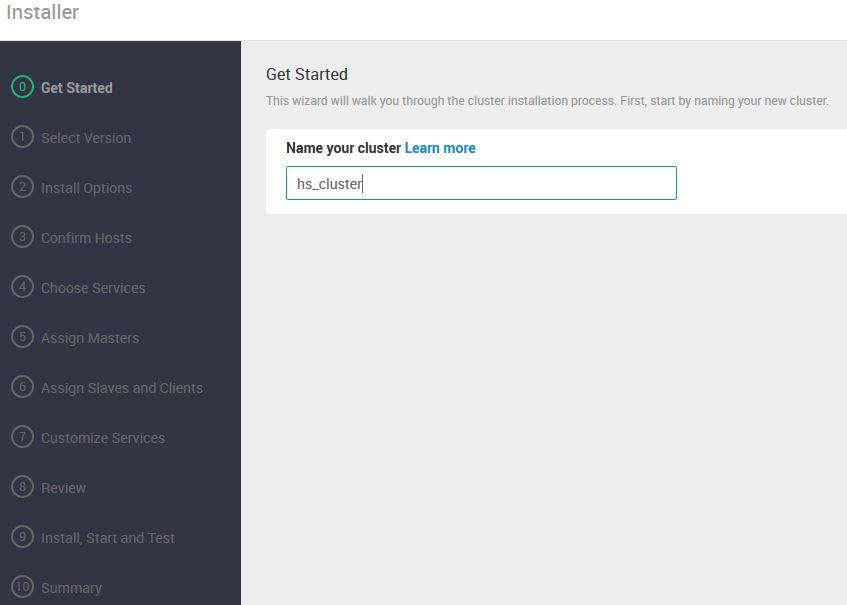
\includegraphics[width=1.3\textwidth]{img/hscluster}
\captionof{figure}{Ambari Wizard Installer}\label{pic:hscluster}
\end{figure}
\noindent Next, we click through the installation routine until the point appears where the cluster nodes are defined. At this point the fact that we are using Ubuntu 18.04 will cause some troubles. If we adding the hosts Ambari is trying to check some dependencies and is running also some check routines. It will fail to add the worker nodes to the cluster since OS is not supported (termination condition). The solution to this problem would be a downgrade of the OS but we don’t have the privileges to do this. So we manually
changed the \textbf{/etc/issue}, \textbf{etc/lsb-release} and \textbf{etc/os-release} file to Ubuntu 16.04 version. Of course, a backup of the original ones has been created as well. After this workaround, the check condition will not fail because Ambari consider our OS as Ubuntu 16.04. Obviously, that’s a dangerous operation, so we change it back to original state after installation has been completed.
In the next step we are choosing our Hadoop services that may be relevant for our data science project. For a start we choose following services: HDFS, YARN, MapReduce2, Tez, Hive, ZooKeeper, Ambari Metrics,
SmartSense, Spark2 and Zeppelin Notebook. Interesting to see is that the proprietary service SmartSense
is the only one that cannot be deselected. We have to install it, even if we don’t want to use it. That’s
certainly not very user-friendly. However, it is simple to add further Apache services on running Ambari
but more difficult to uninstall them so we am do not enable all possible Hadoop services from the
beginning. In addition, some services are not for interest at the moment, hence they would only consume
storage without having a practical effect.\\
After some additional configuration steps we can choose which services should run on master or worker
nodes. Also we have to decide which node should be data node and node manager. In this cluster all four VMs are data nodes as well as node managers. A database connection is also mandatory at this step. Depending on selected services there are several database connections. For instance, the
service Hive needs a working SQL database connection. We can choose between MySQL (MariaDB),
PostgreSQL and Oracle. For a first test, MySQL is used as Hive database. We can change the database
connection setting on Ambari at any time. If the configuration has been finished, a summary with all decisions taken is shown. That’s the last possibility to change a fundamental Hadoop setting. It is worth to check all configurations carefully. Afterwards there is no go back option and the uninstall routine of Ambari is complicated and might lead to tremendous work of removing operations. That is also negative criteria of HDP and Ambari. As soon as the installation completes we can switch to the Ambari monitor. Unfortunately, almost all
selected services were offline or could not start properly. A deeper investigation showed that there were
some permission problems with HDFS and the Hadoop user. The HDFS folder was only for root user but
not for user \glqq Hadoop\grqq. With the command \textbf{chown -R hdfs:hadoop /hadoop/hdfs} the correct permissions could be granted.\\
Another problem was that YARN could not start the name nodes due to connection refused error
messages. As \textbf{netstat -tupln | grep 50070} shown the service was only running for localhost address. After changing the binding address to \textbf{0.0.0.0} on HDFS, the communication between the cluster nodes was working and the name nodes could properly start. However, after fixing this issue, the most services were running. The community of Hortonworks was quite helpful in this case. We got an answer within four hours whereas for getting an answer in Cloudera’s community took three times longer.\\
The data node of the master node was not running correctly. It could be started from Ambari and after
few seconds the data node went offline. A look at the error log of this node showed that the cluster id was already used by another node. Removing the HDFS data folder of the data node solved this issue because
afterwards it generates a new cache file with a new cluster id.\\
The following screenshot shows a (successfully) completed Ambari and HDP installation on our VMs.
\begin{figure}[H]
\hspace{-3.4cm}
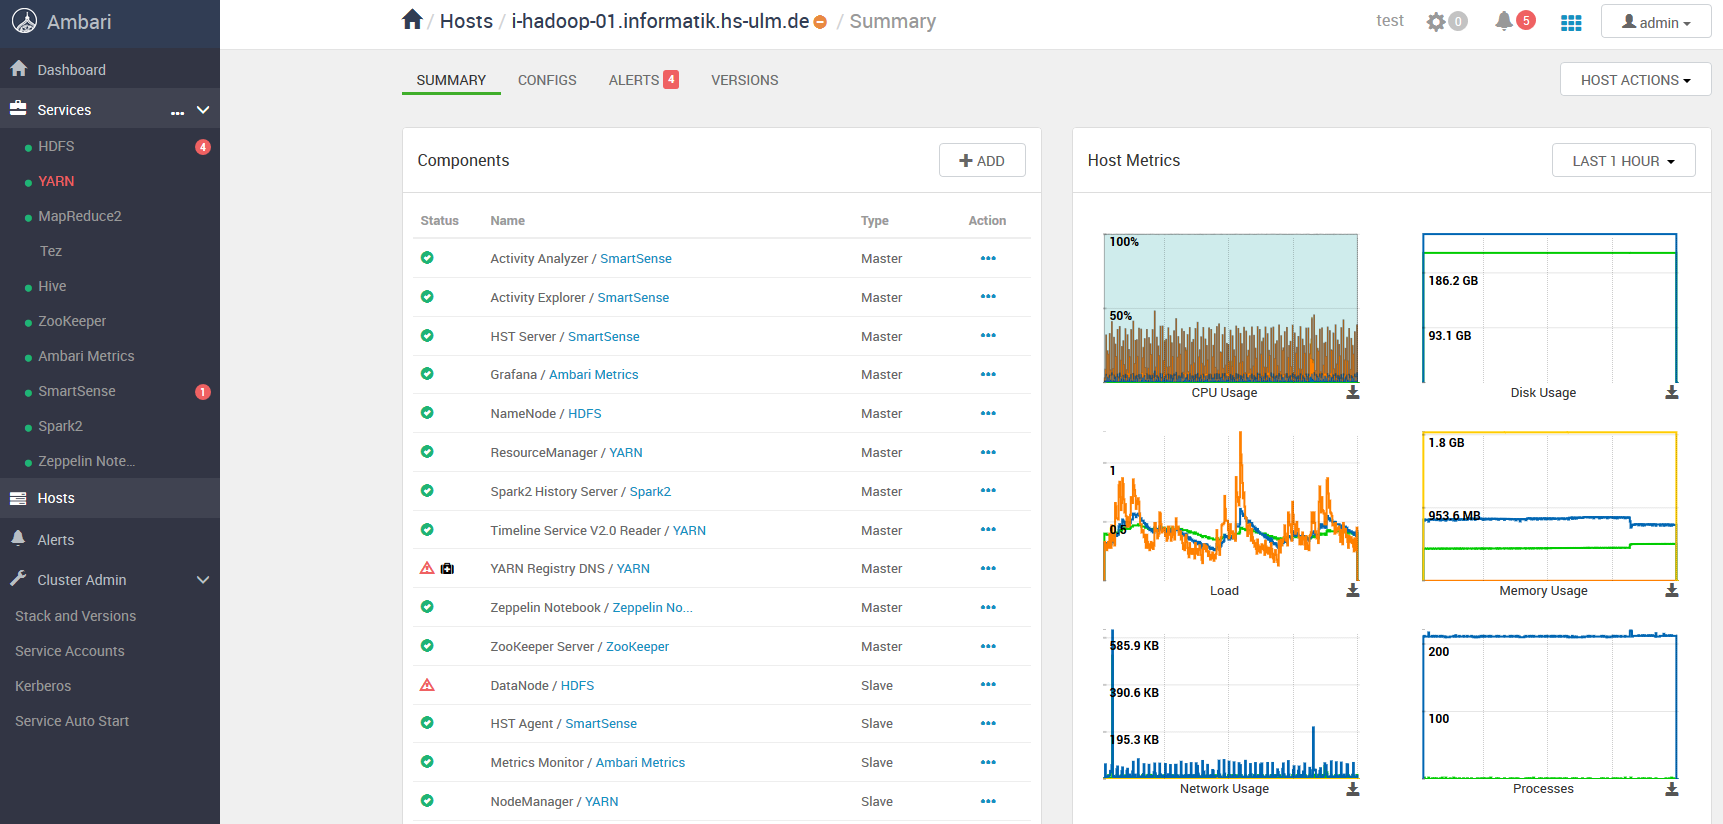
\includegraphics[width=1.5\textwidth]{img/ambari}
\captionof{figure}{Ambari Surface, Host metrics on master node}\label{pic:ambari}
\end{figure}
\noindent Ambari has been set up and most Hadoop services are running (see Figure \ref{pic:ambari}). Ambari shows lot of statistics that might be helpful for cluster management. We can control each service and either turn it off or set it into a maintenance mode. The ladder one encapsulates the service without influencing other services (high availability). Overall, Ambari is a powerful Hadoop cluster management tool that has lot of control options and supervising tools but also lacks in removing services and usability (e.g. no Ubuntu 18.04 support, only Python 2.7.x support, etc). The fact, that there is no official uninstaller from Hortonworks makes HDP with Ambari a risky installation. On the other hand, it is completely open source and has a strong community. Furthermore, HDP 3.0.1 comes up with a bunch of useful Hadoop services and well documentation so that we will likely stay on HDP.\\ Now it is time to run some MapReduce jobs on our newly created Hadoop cluster. 
\subsection{Run MapReduce Jobs}
With four workers (master is also a worker node) a significant speed advantage over single computing should be achieved. First, with a MapReduce job, the accuracy of the decimal places of PI is determined using the quasi Monte Carlo method. This MapReduce job is also offered by the Apache foundation (Source). In the console of the master node the MapReduce job can be started with \acs{yarn} as
follows:
\begin{lstlisting}[language=bash,breaklines=true]
yarn jar /usr/local/hadoop/share/hadoop/mapreduce/hadoop-mapreduce-examples-
3.1.1.jar pi 16 1000
\end{lstlisting}
The \emph{PI job} calculates 16 maps where each map process contains 1000 samples. After a short time, the job is finished and the following output is achieved:
\begin{figure}[H]
\hspace{1.2cm}
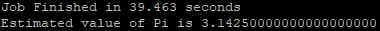
\includegraphics[width=0.8\textwidth]{img/job}
\captionof{figure}{PI Quasi Monte Carlo method executed as Cluster job}\label{pic:job}
\end{figure}
\noindent The same test has been performed with two worker nodes (i.e. two of the four workers were temporarily disabled via Ambari). After that the job took much longer (about 56 seconds). This shows that the Hadoop cluster works and already has a performance advantage over single computing. The next test was a simple WordCount job in Java that calculates the frequency of unique words in an input file distributed across the cluster. A MapReduce job consists of at least a mapper method, a reducer method and a driver method which is often the start method. Before executing the new job one has to put the file of interest on Hadoop’s HDFS. This is simply done as shown below:
\begin{lstlisting}[language=bash,breaklines=true]
hadoop fs -put big.txt
\end{lstlisting}
The put command will upload the file into the HDFS (i.e. it is stored fault-tolerant and replicated 3 times). After that, the following command runs a WordCount job on this text file:
\begin{lstlisting}[language=bash,breaklines=true]
hadoop jar hadoop-mapreduce-examples-3.1.1.jar wordcount wordcountFile big.txt
\end{lstlisting}
Note that now \glqq Hadoop\grqq is used, which starts also the YARN service. There is no difference between executing this with the Hadoop or YARN command. (Although latter is newer and should be used). The output of the \glqq reduced\grqq file looks like figure \ref{pic:words}.
\begin{figure}[H]
\hspace{5.2cm}
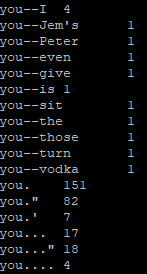
\includegraphics[width=0.2\textwidth]{img/words}
\captionof{figure}{Output of WordCount job}\label{pic:words}
\end{figure}
\noindent Quick to recognize that the words were separated and counted by spaces. In fact, the input text was split
afterwards and each word was mapped as "key value pair", where the key in this case is the word. The
original text file was 6.4 MB, while the newly created file is only 0.93 MB in size. This shows another
potential benefit of the cluster, namely the possible separation of files to minimize the total size of the initial data set. The running time was around 10 seconds. The same job has been executed locally on a
commodity Windows client in NetBeans as well and it took around 8 minutes. There is a plenty of further typical MapReduce jobs (e.g. terasort, randomwriter, sudoko, etc), but for an evaluation these two jobs should already show that the cluster is working apparently faster than a single node.
\subsection{HDP Issues}
Due to the workaround in Chapter \ref{intallhadoop}, a few services could not start properly. Also, permissions for some subfolders were set incorrectly, hence permission denied errors occurred when running the services. During the test phase some other problems were discovered, which are described below. Table \ref{tab:issues} also shows the solution that was found to resolve these issues.
%first part of table issues!
\begin{table}[H]
\hspace{-2.0cm}
\begin{tabular}{|p{4.4cm}|p{12.4cm}|}
	\hline
	\textbf{Issue} & \textbf{Solution} \\ \hline
	No starting NameNodes, Connection
refused. & Go to HDFS$\rightarrow$ Filter at https
0.0.0.0 and \newline localhost address on master node \newline http
127.0.0.0:50070 $\rightarrow$ 0.0.0.0:50070\newline Hive could not start on Node 2 since database was missing (mysql) Permission on HDFS was set to root and not to user hadoop
\\ \hline
Wrong Permissions on HDFS & tail hadoop-hdfs-namenode\newline
chown -R hdfs:hadoop /hadoop/hdfs \\ \hline
Hive Database not found on i-hadoop-02 & \begin{itemize}[noitemsep,leftmargin=*] 
\item Start mysql
\item Show databases;
\item create database hive;
\item CREATE USER 'hive'@'localhost' IDENTIFIED BY 'hive';
\item GRANT ALL PRIVILEGES ON . TO 'hive'@'localhost';
\item CREATE USER 'hive'@'\%' IDENTIFIED BY 'hive';
\item GRANT ALL PRIVILEGES ON . TO 'hive'@'\%';
\item GRANT ALL PRIVILEGES ON . TO 'hive'@'localhost' WITH GRANT OPTION;
\item GRANT ALL PRIVILEGES ON . TO 'hive'@'\%' WITH GRANT OPTION;
\item FLUSH PRIVILEGES;
\end{itemize}
\\ \hline
Bind address in mysql-conf (0.0.0.0): & \begin{itemize}[noitemsep,leftmargin=*] 
\item netstat -tupln | grep 3306
\item Nano /etc/mysql/mysql.conf
\item Change bind-address to 0.0.0.0
\item Systemctl mysql restart
\item Service mysql restart
\end{itemize}
\\ \hline
YARN DNS Server not starting,\newline connection refused & \begin{itemize}[noitemsep,leftmargin=*] 
\item Change Port 53 to other Port
\item Set right permissions on YARN folder
\end{itemize}
\\ \hline
\end{tabular}
%\caption{Issues}
\label{tab:issues}
\end{table}
%second part of tabel issues
\begin{table}[H]
\hspace{-2.0cm}
\begin{tabular}{|p{4.4cm}|p{12.4cm}|}
	\hline
	\textbf{Issue} & \textbf{Solution} \\ \hline
Master Node worker is not starting (Conflicting cluster id) & \begin{itemize}[noitemsep,leftmargin=*] 
\item Stop service
\item sudo wget archive.apache.org/dist/zeppelin/zeppelin-0.8.0/zeppelin-0.8.0-bin-all.tgz
\item sudo tar -xf zeppelin-0.8.0-bin-all.tgz
\item Move interpreter to /usr/hdp/current/zeppelin-server/interpreter/
\item sudo chown -R zeppelin:zeppelin/usr/hdp/current/zeppelin-server/interpreter/
\item Start service
\end{itemize}
\\ \hline
Umask is changing from 0022 to 0002 & \begin{itemize}[noitemsep,leftmargin=*] 
\item sudo gedit ~/.bashrc
\item Add line umask 022
\item Logout and login
\end{itemize}\\ \hline
FAILED [2018-12-0813:36:00.609]\newline java.io.IOException:\newline mkdir of /hadoop/yarn/local/filecache/60\_tmp failed & \begin{itemize}[noitemsep,leftmargin=*] 
\item YARN permissions
\item sudo chown yarn yarn
\item sudo chmod 750 yarn
\end{itemize}
\\ \hline
\end{tabular}
\caption{Problems and solutions of HDP}
\label{tab:issues}
\end{table}
\noindent The described problems and their solutions of table \ref{tab:issues} show that many setting options should be checked carefully during the Ambari installation routine (e.g. if a MySQL database exists). Furthermore, it can be assumed that most of these issues can be explained by the \glqq officially\grqq unsupported operating system version. However, after the fix, all Hadoop services in Ambari had a green status point. 
\subsection{Recommendation}
The evaluation showed that Hortonworks with the Hadoop distribution HDP is best suited for our goals.
Ambari provides an efficient, comprehensive cluster management tool for monitoring and controlling the
Hadoop cluster. In addition, an active community and complete open source freedom can convince more
than its competitors. Although all three Hadoop distributions may have their individual advantages and
disadvantages (see evaluation matrix in figure \ref{pic:matrix}), HortonWorks was able to convince us due to the reasonably good documentation and the easy to follow Ambari installation routine. It should be noted, however, that the Cloudera Manager installation wizard also has good documentation and a comparable installation effort. However, we liked the Ambari interface more than the CDH one. In addition, Cloudera's pricing is not entirely transparent and third-party module integration is rather difficult. For example, since CDH 5.11 there has been a proprietary \glqq data science workbench\grqq service replacing Jupyter and IPython notebooks. HortonWorks, on the other hand, offers Zeppelin notebooks that resemble the famous Jupyter notebooks. Apart from that, Jupyter could also be installed as a third module during the test phase of HDP, even though such installations are naturally risky and are not officially supported by HortonWorks.
\\It is interesting that MapR, HortonWorks and Cloudera offer Docker images for immediate testing. For
example, MapR offers a VMware image free of charge. However, all these packages have the disadvantage
that they only have a single node cluster and limited functionality. For example, I could not select any
services or create new ones in MapR and the function to add more worker nodes to the existing cluster
was also not available. Therefore, such images or sandboxes are ideal for a quick check of the user interface and some standard functions, but rather insufficient for a complete range of functions or a productive system.\\
In conclusion it can be said that all three Hadoop distributions would meet the requirements of a big data
project or our project perfectly, but HortonWorks could simply convince more with the overall score than
the more commercially oriented counterparts. Ultimately, the performance also depends on the hardware
of the individual cluster nodes. Due to a low physical RAM, MapReduce jobs even with MapR's high
performance HDFS would be processed slowly by YARN and would probably lead to
\emph{MemoryOutOfExceptions}. Because Hadoop and every single service on top needs resources and these can
quickly bring a commodity computer with standard equipment to its knees. In any case, the HDP cluster is
ready for big data tasks and will be extremely helpful to us in the further course of the project. With Apache Spark, even better performance values might be achieved due to its \glqq in-memory\grqq engine. The test cluster with the four VMs also showed which special features and requirements you should pay attention to (e.g. operating system version).
\subsection{Hadoop Rollout}
For the Hadoop rollout ten fat clients each with 32 GB RAM and 2 TB HDD as well as 128 GB SSD
have been used. The nodes were connected with a 48port Gigabit switch and a routable gateway,
so that all nodes were in a single local domain. For various reasons (e.g. security) the installation
of a hypervisor (Proxmox) has proven to be successful, with which any number of VMs can be
generated and configured (figure \ref{fig:figure1_proxmox}).
\begin{figure}[H]
\hspace{-2.8cm}
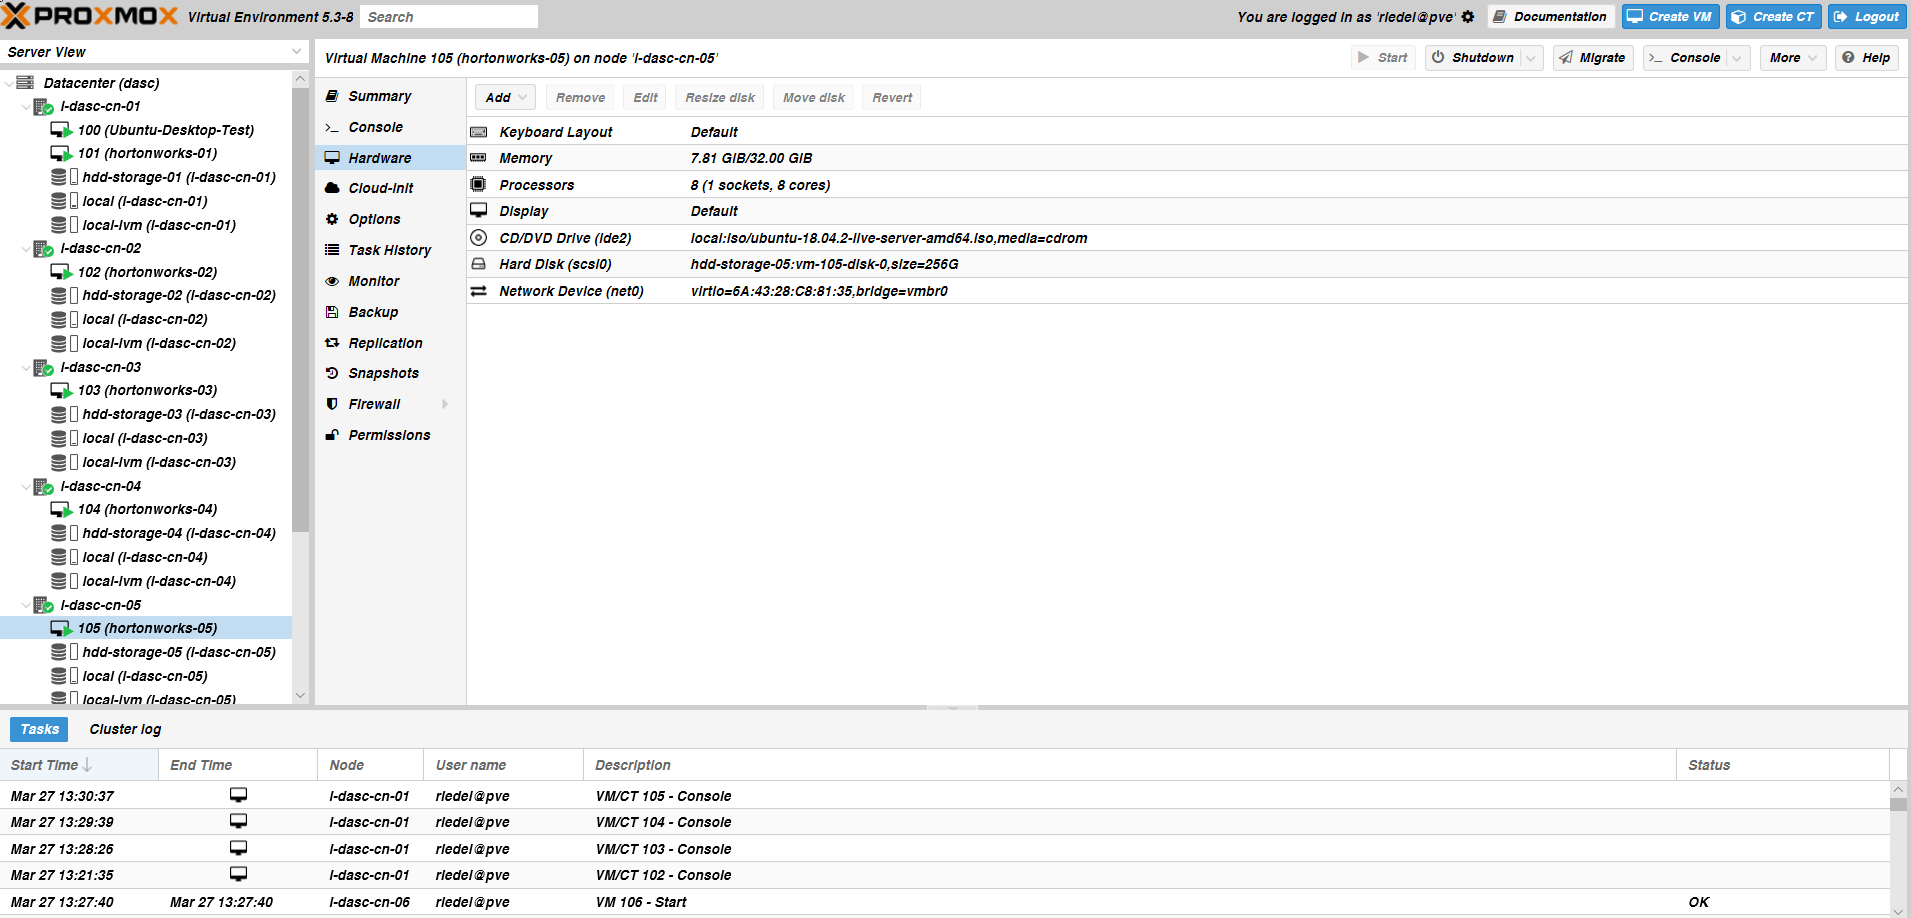
\includegraphics[width=1.4\textwidth]{img/figure1_proxmox}\label{fig:figure1_proxmox}
\captionof{figure}{Proxmox surface}\label{fig:figure1_proxmox}
\end{figure}
A VM with Ubuntu Server 18.04.02 LTS was installed for each node. Each VM got an allocated
memory of 256 GB and a reserved memory for the Logical Volume Manager (LVM). Furthermore,
sparse files were allowed and VirtIO SCSI interfaces were configured for the individual VMs, which
should guarantee maximum VM performance (\cite{RN1}).\\\\
For the first rollout attempt, six cluster nodes were configured for Hadoop. The remaining four nodes
were later added to the existing Hadoop cluster via Ambari surface. The chosen Hadoop stack
was HDP from Hortonworks, as already explain in the Hadoop evaluation part of this work. In
addition, Webmin was installed on the master node, which offers extensive monitoring services
on the node. For example, the current CPU load, memory usage, kernel information and much
more can be displayed. Figure \ref{fig:figure2_webmin} shows the surface of Webmin. Although monitoring services
are also offered with Ambari Metrics, they run on top of Hadoop and can only be called when
Ambari is running as well (\cite{RN2}).
\begin{figure}[H]
\hspace{-3.2cm}
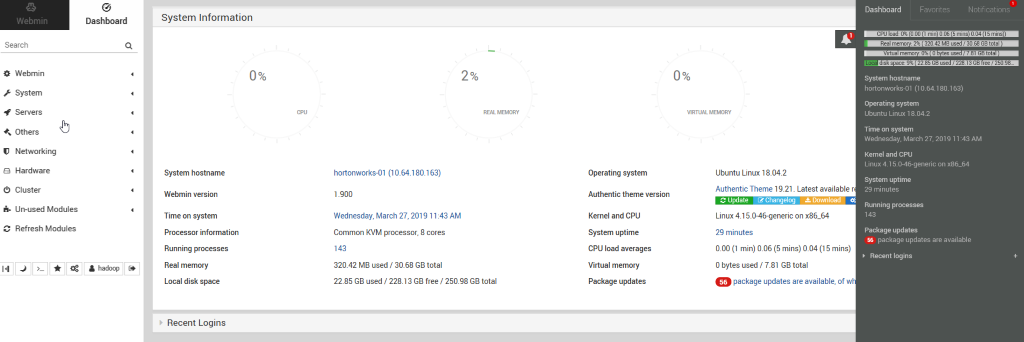
\includegraphics[width=1.5\textwidth]{img/figure2_webmin}\label{fig:figure2_webmin}
\captionof{figure}{Webmin dashboard}\label{fig:figure2_webmin}
\end{figure}
Before the Ambari Wizard can install HDP, some pre-configurations have to be done on each VM.
On the one hand, \glqq ulimit\grqq must be set to at least 10000, because Ambari installs several thousand
dependencies. On the other hand, a password-less ssh authentication is necessary so that the
master node can connect to its worker nodes without entering a password. In addition, the master
node must be able to execute \glqq sudo\grqq commands without entering a password. This can be done
by editing the \glqq visudo\grqq file and adding \glqq username ALL=(ALL) NOPASSWD:ALL\grqq . Another
necessity is to add the IP addresses and hostnames of all cluster nodes under \glqq /etc/hosts\grqq . This
must also be done on each node individually. The following table shows the current host
configurations of a worker respectively slave node:
\begin{table}[H]
\centering
\begin{tabular}{|l|l|}
\hline
\textbf{IP-Address} & \textbf{List of hostnames} \\ \hline
10.64.180.163 & \begin{tabular}[c]{@{}l@{}}hortonworks-01.dasc.cs.thu.de\\ hortonworks-01\end{tabular} \\ \hline
10.64.83.106 & \begin{tabular}[c]{@{}l@{}}hortonworks-02.dasc.cs.thu.de\\ hortonworks-02\end{tabular} \\ \hline
10.64.79.161 & \begin{tabular}[c]{@{}l@{}}hortonworks-03.dasc.cs.thu.de\\ hortonworks-03\end{tabular} \\ \hline
10.64.227.154 & \begin{tabular}[c]{@{}l@{}}hortonworks-04.dasc.cs.thu.de\\ hortonworks-04\end{tabular} \\ \hline
10.64.159.100 & \begin{tabular}[c]{@{}l@{}}hortonworks-05.dasc.cs.thu.de\\ hortonworks-05\end{tabular} \\ \hline
10.64.204.57 & \begin{tabular}[c]{@{}l@{}}hortonworks-06.dasc.cs.thu.de\\ hortonworks-06\end{tabular} \\ \hline
\end{tabular}
\caption{etc/hosts of a worker node}
\label{tab:hadooprollout}
\end{table}
Databases (Hive, Ranger, Druid...) are created by the Ambari Wizard as PostgreSQL databases
automatically. Java as well as a corresponding JDBC connector are required for the individual
services to execute database statements. The node \glqq hortonworks-01\grqq (see table \ref{tab:hadooprollout}) is both a
master and a worker node. On the master node the Ambari Wizard installs Ambari server. The Ambari Agents, which are required for communication in the cluster, are installed on each worker
node. Afterwards, the Ambari Wizard can be called under the following URL:\\
\emph{hortonworks-01.dasc.cs.thu.de:8080}.\\
The installation routine guides the user through all necessary steps. It
is important that the Ambari agents are installed on the individual worker nodes, otherwise the
Ambari Wizard cannot add the nodes to the cluster. The most important step is probably the
selection of the HDP services. Similar to the evaluation step with the VMs described in section \ref{intallhadoop},
the identical service packages were selected, i.e. YARN+MapReduce2, Tez, Hive, HBase, Pig,
ZooKeeper, Ambari Metrics, Spark2, Zeppelin and SmartSense. But also some new services were
added for the production cluster: Storm, Accumulo, Infra Solr, Atlas and Kafka. Since the cluster
is to become a long-lived high performance cluster, it might reasonable to rollout the playground
for distributed streaming platforms like Kafka or Storm which can be used for streaming analytics
use-cases.\\\\
Selection of services that are running on top of Hadoop is an important part of the Hadoop cluster
setup process. Following services have been chosen from the HDP stack: \\
all 6 virtualized nodes are DataNodes (workers) and each have a YARN NodeManager (which takes care of the resource
distribution and monitoring of a node).\\
Furthermore, all master components run on \glqq hortonworks-01\grqq . However, the cluster is fault-tolerant, so if the master node fails, the worker \glqq hortonworks-02\grqq
becomes the active master. This is made possible by the secondary NameNode service that runs
on another worker node.\\\\
Once the individual accounts have been created for the different services, a final briefing is
performed by Ambari before the cluster is started. A useful feature of Ambari is to download the
complete configuration as a JSON template \cite{RN3}. This makes another Hadoop installation much
easier because the template can be reused.\\\\
This time, the installation process was done without any problems. HortonWorks (HDP 3.1.0)
supports recently Ubuntu 18.04.02 LTS which makes tweaking of the operating system
superfluous. Initializing and starting Hadoop services may take a few hours, depending on the size
of cluster. The productive cluster now runs on Ambari 2.7.3.0 and HDP 3.1.0. By default, Zeppelin
comes with a Python 2 kernel. However, it is possible to switch to the Python 3 kernel (IPython
with Python 3.x).\\\\
The Ambari interface is intuitive to use. A first look at Ambari Metrics showed that the services
worked properly and all workers in the cluster were active. Only YARN Registry DNS did not seem
to start due to a connection refused error because Hadoop relies heavily on a functioning DNS
server \cite{RN4}. However, changing the YARN RDNS Binding Port from \glqq 53\grqq to \glqq 5300\grqq solved the problem.\\ Remark: the same issue happened in the evaluation part where a port conflict prevented a successful start of the Ambari server.
\\\\
The physical hardware configuration of the cluster consists of 10 fat nodes, as figure \ref{fig:figure3_hadoop} shows.
\begin{figure}[H]
\centering
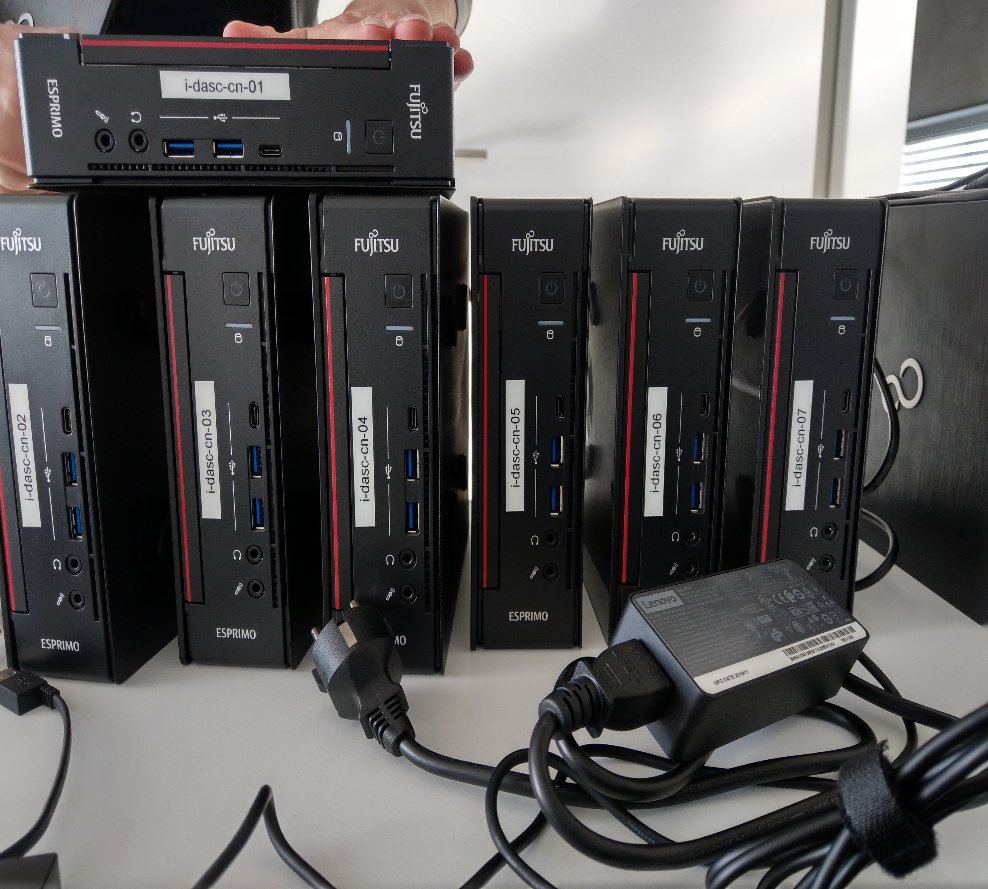
\includegraphics[width=0.6\textwidth]{img/figure3_hadoop}\label{fig:figure3_hadoop}
\captionof{figure}{Physical Hadoop cluster}\label{fig:figure3_hadoop}
\end{figure}
These nodes were locally connected with a switch and a gateway so that all nodes could
communicate with each other. Unfortunately, access outside the intranet was not possible, as the
necessary infrastructure measures on the part of the data center are still pending. In principle,
however, it would be possible to access the cluster from outside using VPN and a reliable
authentication method.\\\\
First tests with the six configured Hadoop nodes could be carried out successfully. These tests were
based on the Zeppelin notebooks from the previous data profiling chapter \ref{dp1}, which already worked
successfully in the virtual cluster. Compared to the virtual cluster this time the execution was much
faster, because more RAM was available and more workers (six! instead of four) were used.\\\\
Thus the cluster (figure \ref{fig:figure3_hadoop}) is in an operational and ready configured state. Of course, it is possible
that a service may fail on its own or no longer run properly over time. In the evaluation phase, for
example, it was shown that the YARN Timeline service fails more frequently. Usually, however, a
restart of the corresponding service via the Ambari interface is sufficient. Most Hadoop services also run autonomously, i.e. a corrupt service cannot block other running services (exception: HDFS). With the new ready to use Hadoop cluster, further data profiling action of the bicycle data can now be performed in the cluster.